\documentclass[11pt,a4paper]{article}
\usepackage[margin=2.2cm]{geometry}
\usepackage[T1]{fontenc}
\usepackage{lmodern}
\usepackage{booktabs}
\usepackage{tabularx}
\usepackage{array}
\usepackage{amsmath}
\usepackage{graphicx}
\usepackage{xcolor}
\usepackage{enumitem}
\usepackage{float}
\usepackage[hidelinks]{hyperref}
\setlist{nosep,leftmargin=1.4em}
\newcolumntype{L}{>{\raggedright\arraybackslash}X}
\graphicspath{{figures/}{../figures/}}

\title{Methodology and Preliminary Results\\[4pt]
\large Controller CPU budgets and forecasting overhead in predictive Kubernetes autoscaling}
\author{Saad Azhar (i230822) \and Ali Ramish (i230651)\\[2pt]
\small Cloud Computing Research --- Cutoff 3 \quad Group 35 \quad Supervisor: Basharat Hussain\\
\small FAST NUCES Islamabad}
\date{November 2026}

\begin{document}
\maketitle

\begin{abstract}
We operationalise the research question of whether Prophet--LSTM hybrid forecasters can fit inside
Kubernetes controller CPU budgets while producing timely, causally valid forecasts that improve on the reactive
Horizontal Pod Autoscaler (HPA). We built a budget-aware KEDA external scaler: forecasts run in a worker process
under a CPU limit (100m--500m) and a deadline equal to the control period, with a persistence fallback. Around it
we built a trace-driven simulator and a live kind/Prometheus testbed, and ran four experiments on NASA-HTTP and
WorldCup98 traces.
(E1) The base paper's evaluation is leaky: under a causal protocol the hybrid's RMSE is 43\,\% (NASA) and 40\,\%
(FIFA) higher than reported, and it is beaten by AR(10) on both traces and by persistence on FIFA.
(E2) Per-decision inference fits every budget (266\,ms of CPU and 2.9\,s p95 latency at 100m; no late
forecasts at a 15\,s period). The binding costs are cold start (270\,s at 100m), memory ($\approx$\,0.7\,GB) and
re-fitting, which cannot run inside the budget.
(E3, E4) Request-rate scaling reduces under-provisioning compared with the CPU HPA on bursty and ramping load
(live: $\Theta_U$ 12.1\,\%$\to$0.7\,\%, SLO violations 1.11\,\%$\to$0.06--0.54\,\%, for 21--25\,\% more
pod-minutes). A persistence forecaster achieves the same gain, and Prophet alone fails on flash crowds (90\,\% SLO
violations). These are preliminary single-run results.\\[4pt]
\textbf{Reproducibility:} The code and reproducibility materials for this study are publicly available at: \url{https://github.com/Saadx-git/Cloud_project_I230822_I230651}
\end{abstract}

\tableofcontents
\newpage

%=====================================================================
\section{Research Question and Objectives}
Cutoff~2 showed that the published accuracy of the Prophet--LSTM autoscaler of Guruge and
Priyadarshana~\cite{guruge2025} comes from a non-causal evaluation. The forecast for minute $t{+}1$ is scored
against minute $t$. Once this is corrected, the hybrid loses most of its advantage over simple models. The paper
also never measures the forecaster \emph{inside} a running controller. Cutoff~3 therefore operationalises the
research question:

\begin{quote}\itshape
RQ: Can predictive autoscaling models (Prophet--LSTM hybrids) fit within Kubernetes controller CPU budgets
while producing timely, causally valid forecasts that improve scaling decisions compared with the reactive HPA?
\end{quote}

\begin{enumerate}[label=O\arabic*]
\item Quantify forecast quality at $t{+}1$ under a strictly causal protocol, and the inflation caused by the
      leaky protocol (E1).
\item Measure the controller-side cost of each forecaster as a function of the controller's CPU limit:
      CPU per decision, latency against the control period, cold start, memory and re-fitting (E2).
\item Compare end-to-end scaling quality of HPA and predictive scalers that share one replica policy, on four
      workload scenarios, including budget-induced late forecasts (E3, trace-driven).
\item Validate the comparison on a live Kubernetes cluster with KEDA and a CPU-limited scaler (E4).
\end{enumerate}

%=====================================================================
\section{Methodology}
\subsection{System under test}
Figure~\ref{fig:arch} summarises the framework. Its components:
\begin{itemize}
\item \textbf{Workload service} (\texttt{app/}). A CPU-bound HTTP service in which every request performs a
      fixed PBKDF2 computation. CPU utilisation is therefore proportional to the request rate, and a pod has a
      well-defined capacity $C$ (requests/s at 100\,\% of its CPU request).
\item \textbf{Load generator} (\texttt{loadgen/replay.py}). It replays a trace slice open-loop with Poisson
      arrivals at $\lambda = y_{\text{trace}}\cdot s$. One trace minute is replayed in 15\,s of wall time.
\item \textbf{Monitoring}. Prometheus scrapes the service every 5\,s; metrics-server runs at 15\,s resolution
      for the HPA.
\item \textbf{Predictive scaler} (\texttt{scaler/}). A KEDA \emph{external scaler} (gRPC). Its control loop
      runs once per control period $P$:
      \begin{enumerate}
      \item it reads the request rate of the last period from Prometheus;
      \item it sends a forecast request to a worker process that holds the model;
      \item it waits at most $D$ seconds for the answer;
      \item it publishes the forecast, which KEDA's HPA turns into replicas.
      \end{enumerate}
      The gRPC \texttt{GetMetrics} call only returns the latest published value, so KEDA's own timeouts never
      interact with inference time.
\end{itemize}

\begin{figure}[H]\centering\small
\begin{tabular}{c}
\fbox{\begin{minipage}{0.92\textwidth}\centering
\texttt{replay.py} (trace $\times s$, 15\,s/min) $\longrightarrow$ \textbf{Service} \texttt{work} (Deployment, 100m req / 200m lim per pod)\\[2pt]
$\downarrow$ \texttt{app\_requests\_total} \qquad\qquad\qquad\qquad\qquad $\downarrow$ CPU usage\\[2pt]
\textbf{Prometheus} (5\,s scrape) \qquad\qquad\qquad\qquad \textbf{metrics-server} (15\,s)\\[2pt]
$\downarrow$ \qquad\qquad\qquad\qquad\qquad\qquad\qquad\qquad\qquad $\downarrow$\\[2pt]
\textbf{Budgeted scaler} [CPU limit 100m--500m] \qquad\qquad \textbf{HPA} (B1, CPU 70\,\%)\\
observe $\to$ worker.forecast (deadline $D$) $\to$ late? fallback $y_t$ \& restart worker\\
$\downarrow$ gRPC \texttt{GetMetrics} (forecast req/s)\\
\textbf{KEDA} $\to$ HPA (\texttt{AverageValue} $=0.7C$) $\longrightarrow$ \texttt{work} replicas
\end{minipage}}
\end{tabular}
\caption{Experimental framework (live setting, E4). E2 runs the same scaler image under \texttt{docker --cpus};
E3 replaces the cluster with a trace-driven simulator that implements the same replica policy.}\label{fig:arch}
\end{figure}

\subsection{Compared autoscalers and the shared replica policy}
To isolate the effect of the \emph{signal}, all autoscalers use one replica policy:
\[
  N_{t+1}=\Big\lceil \frac{\text{signal}}{0.7\,C} \Big\rceil,
\]
with the HPA's 10\,\% tolerance, immediate scale-up, and a scale-down stabilisation window of 5 control periods
(the Kubernetes default of 300\,s at a 60\,s step; 75\,s in the time-compressed live runs).
\begin{itemize}
\item \textbf{B1 -- HPA (reactive).} The signal is the CPU utilisation observed in period $t$. It saturates at
      the pod CPU limit (200\,\% of the request), as in a real cluster.
\item \textbf{B2 -- Prophet scaler.} The signal is Prophet's $\hat y_{t+1}$, with the released notebook's
      hyperparameters: changepoint prior 5.1, seasonality prior 30, weekly/daily Fourier orders 20/50, and
      linear (NASA) or flat (FIFA) growth.
\item \textbf{Proposed -- budgeted Prophet--LSTM.} The forecast is
      $\hat y_{t+1} = \hat y^{P}_{t+1} + \mathrm{LSTM}(y_t-\hat y^{P}_t)$, using the released architecture
      (2$\times$50 LSTM, look-back 1). It runs under a CPU limit of 100m--500m and a deadline $D=P$. If the
      deadline is missed, the persistence fallback $y_t$ is used and the worker is killed and re-spawned.
      Each model is evaluated in two implementations:
      \begin{itemize}
      \item \emph{as released}: \texttt{Prophet.predict} with 1000 uncertainty samples, and
            \texttt{keras.Model.predict};
      \item \emph{optimised}: no uncertainty sampling, and a direct model call.
      \end{itemize}
\item \textbf{Lightweight references.} Persistence, 5-minute moving average, seasonal naive (1 day), and
      AR(10) fitted by least squares.
\end{itemize}

\subsection{Causal evaluation protocol}
Models are trained on the chronological first 70\,\% of each trace and evaluated on the remaining 30\,\%, as in
the base paper. Two corrections are made, and the original variant is kept for comparison:
\begin{itemize}
\item \textbf{Alignment (fixes F1).} A forecast is written to the row it forecasts, and its inputs are limited
      to rows before it. The base paper's alignment is retained as a labelled \emph{leaky} variant.
\item \textbf{Scaler fitting (fixes F2).} The residual Min--Max scaler is fitted on training residuals only.
\end{itemize}
In the live scaler, Prophet is queried at the \emph{trace} timestamp of the replayed minute. This avoids the
30-year extrapolation of the released scaler (F4).

\subsection{Workloads and scenarios}
Both traces are the per-minute request counts released with the base paper (NASA-HTTP, Jul--Aug 1995;
WorldCup98, Apr--Jul 1998). Four scenarios are cut from the test splits (Table~\ref{tab:scen}). Each is
preceded by 1500 minutes of observed history, which serves as forecaster warm-up.

\begin{table}[H]\centering\small
\begin{tabular}{llllrrrrrrr}
\toprule
Scenario & Trace & Window & Type & Min & Mean & Max & CV & Peak/mean & p99 step & ACF(1) \\
\midrule
steady & NASA & 1995-08-26 00:00 -- 00:00 & steady & 1440 & 22 & 87 & 0.59 & 3.96 & 650\% & 0.571 \\
ramp & FIFA & 1998-07-07 09:51 -- 16:32 & gradual ramp & 401 & 15,450 & 21,827 & 0.25 & 1.41 & 14\% & 0.981 \\
bursty & FIFA & 1998-07-07 18:00 -- 23:00 & bursty & 300 & 95,099 & 229,426 & 0.60 & 2.41 & 12\% & 0.998 \\
diurnal & NASA & 1995-08-22 00:00 -- 00:00 & diurnal & 1440 & 40 & 140 & 0.61 & 3.49 & 307\% & 0.744 \\
\bottomrule
\end{tabular}

\caption{Workload scenarios (test split only). CV: coefficient of variation; p99 step: 99th percentile of the
absolute minute-to-minute change.}\label{tab:scen}
\end{table}

\subsection{Metrics}
\begin{itemize}
\item \textbf{Forecast quality} at $t{+}1$: RMSE, MAE and $R^2$, computed in raw requests/minute for both traces.
\item \textbf{Controller overhead}:
      \begin{itemize}
      \item CPU time per decision (\texttt{process\_time}, all threads);
      \item wall latency (p50/p95/max);
      \item cold start (import, model load and first call);
      \item resident memory;
      \item CFS throttling ratio;
      \item share of the period's CPU budget used per decision;
      \item cost of re-fitting Prophet on the last 7 days plus one LSTM epoch.
      \end{itemize}
\item \textbf{Scaling quality}. The under/over-provisioning metrics of the base paper's evaluation notebook,
      with $r_t$ the demand and $p_t$ the provisioned capacity ($=$ ready pods $\times\,0.7C$):
      \[
      \Theta_U=\tfrac{100}{T}\sum_t \tfrac{\max(r_t-p_t,0)}{r_t},\quad
      \Theta_O=\tfrac{100}{T}\sum_t \tfrac{\max(p_t-r_t,0)}{r_t},\quad
      T_U=\tfrac{100}{T}\#\{r_t>p_t\},\quad T_O=\tfrac{100}{T}\#\{p_t>r_t\}.
      \]
      We also report pod-minutes and the share of time saturated (demand above $N\!\cdot\!C$). In the live runs
      we additionally report the share of requests violating a 500\,ms latency SLO (error, timeout, or
      slower than 500\,ms).
\item \textbf{Timeliness}:
      \begin{itemize}
      \item decision latency against $P\in\{15,30,60\}$\,s;
      \item late-forecast fraction $\Pr[\text{latency}>P]$;
      \item cold start expressed in control periods without a model forecast.
      \end{itemize}
\end{itemize}

%=====================================================================
\section{Experimental Setup}
\subsection{Hardware and software}
\begin{table}[H]\centering\small
\begin{tabularx}{\textwidth}{@{}lL@{}}\toprule
Host & Laptop, Intel Core i5-1035G1 (4 cores / 8 threads, 1.0--3.6\,GHz), 15\,GB RAM, no GPU; Fedora Linux 45, kernel 7.2.15 \\
Container runtime & Docker 29.9.3 (cgroup v2); CPU budgets enforced with CFS quota (\texttt{--cpus} / \texttt{limits.cpu}) \\
Kubernetes & kind v0.27.0, single node, Kubernetes v1.32.2; HPA sync period 15\,s; metrics-server 0.7.2 (15\,s resolution) \\
Autoscaling & KEDA 2.16.1 (external scaler, gRPC); Prometheus 3.2.1 (5\,s scrape) \\
Python & 3.11; prophet 1.5.0 (cmdstanpy 1.3.0), tensorflow-cpu 2.21.0, keras 3.15.1, numpy 2.4.6, pandas 3.0.6, grpcio 1.84.0 (identical to the Cutoff~2 lock file) \\
Seeds & 42 for model training; load generator seed 1; simulator is deterministic \\
\bottomrule\end{tabularx}
\caption{Environment. The Cutoff~2 reproduction used a different laptop (i5-7300U); absolute times are therefore not comparable across the two reports.}
\end{table}

\subsection{Parameters}
\begin{itemize}
\item \textbf{Training.} Prophet--LSTM is trained on the first 70\,\% of each trace: NASA 56{,}977\,min, FIFA
      87{,}709\,min. The LSTM uses 20 epochs, early stopping with patience 5, batch size 16, and Adam.
      Early stopping halted after 6 epochs (NASA) and 16 epochs (FIFA). Training took 205\,s (NASA) and 397\,s
      (FIFA) on 8 threads.
\item \textbf{E2.} 30 decisions per configuration, paced at 1 per second, on consecutive minutes of the
      \texttt{bursty} scenario with 1500 minutes of history. CPU limits are 100m, 250m, 500m, 1000m and
      unlimited. There is one fresh container per configuration, and the cold start is measured inside it.
\item \textbf{E3.} One step is one minute ($P=60$\,s). The pod capacity is normalised so that each scenario's
      peak needs 10 pods at the 70\,\% target. Pod startup delay is 0 (main results) or 1 step (sensitivity).
\item \textbf{E4.} The \texttt{bursty} slice 18:50--20:30 (100 trace minutes, 27.1k$\to$137.6k req/min) is
      replayed at 15\,s per trace minute, scaled so that the peak needs 10 pods. Each workload pod has a CPU
      request of 100m and a limit of 200m. Calibration gave a pod CPU of about 25\,m per request/s, so
      $C\approx4.0$\,req/s and the target is $0.7C=2.8$\,req/s per pod. The HPA target is 70\,\% CPU; KEDA's
      target is 2800 milli-req/s per pod. The control period is 15\,s, the scale-down stabilisation 75\,s, the
      scaler deadline $D=P=15$\,s, and the latency SLO 500\,ms. Runs are executed sequentially on an otherwise
      idle host.
\end{itemize}


%=====================================================================
\section{Preliminary Results}
All numbers below are produced by the scripts in \texttt{cutoff3/experiments/}. The tables are generated
from \texttt{cutoff3/results/} by \texttt{make\_figures.py}.

\subsection{E1: Causal vs.\ leaky forecast accuracy}
\begin{figure}[H]\centering
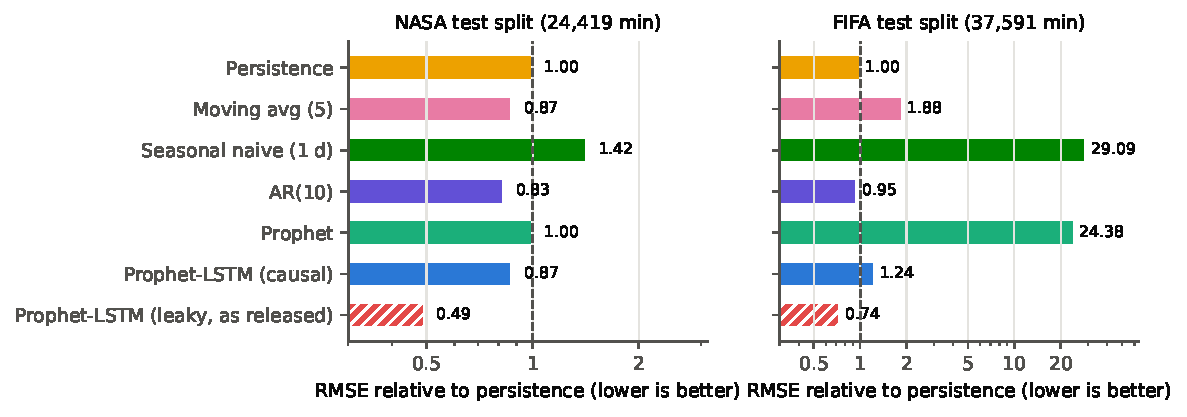
\includegraphics[width=\textwidth]{fig_e1_causal_vs_leaky.pdf}
\caption{One-step-ahead RMSE relative to persistence on the full test splits (log scale). The hatched bar
uses the base paper's mis-aligned evaluation.}\label{fig:e1}
\end{figure}
\begin{table}[H]\centering\small
\begin{tabular}{lrrrrrr}
\toprule
Forecaster & \multicolumn{3}{c}{NASA} & \multicolumn{3}{c}{FIFA} \\
 & RMSE & MAE & $R^2$ & RMSE & MAE & $R^2$ \\
\midrule
Persistence & 16.40 & 12.28 & 0.579 & 763 & 374 & 0.998 \\
Moving avg (5) & 14.32 & 10.81 & 0.679 & 1431 & 454 & 0.994 \\
Seasonal naive (1 d) & 23.35 & 17.46 & 0.147 & 22190 & 6809 & -0.394 \\
AR(10) & 13.58 & 10.32 & 0.711 & 728 & 375 & 0.998 \\
Prophet & 16.37 & 12.56 & 0.581 & 18599 & 9058 & 0.021 \\
Prophet-LSTM (causal) & 14.32 & 10.94 & 0.679 & 944 & 510 & 0.997 \\
Prophet-LSTM (leaky, as released) & 8.10 & 6.28 & 0.897 & 564 & 310 & 0.999 \\
\bottomrule
\end{tabular}

\caption{E1: $t{+}1$ accuracy in raw requests/minute (NASA 24{,}419 and FIFA 37{,}591 test minutes).}\label{tab:e1}
\end{table}

\paragraph{Leakage inflates accuracy.} The leaky evaluation, which writes the forecast for $t{+}1$ into row $t$,
under-states the hybrid's RMSE:
\begin{itemize}
\item NASA: 8.10 instead of 14.32 ($-43$\,\%; $R^2$ 0.897 vs.\ 0.679).
\item FIFA: 564 instead of 944 ($-40$\,\%).
\end{itemize}
The leaky residual ``forecast'' correlates at 0.9997 (NASA) and 0.9996 (FIFA) with the residual of the
\emph{same} row. This confirms the Cutoff~2 finding with independently re-trained models and scalers fitted on
training data only.

\paragraph{Causal ranking.} Under the causal protocol:
\begin{itemize}
\item On NASA the hybrid beats Prophet and persistence (RMSE $-13$\,\%). It only ties a 5-minute moving average
      (14.32 vs.\ 14.32), and \textbf{AR(10)} is more accurate (13.58).
\item On FIFA the hybrid is \textbf{24\,\% worse than persistence} (944 vs.\ 763). Prophet alone explains almost
      none of the variance ($R^2=0.02$), because the flat-growth seasonal model cannot represent the
      match-driven flash crowds. AR(10) is again the most accurate (728).
\end{itemize}
The hybrid's apparent accuracy advantage is therefore an artefact of the evaluation, not of the model.

\subsection{E2: Controller overhead under CPU budgets}
\begin{figure}[H]\centering
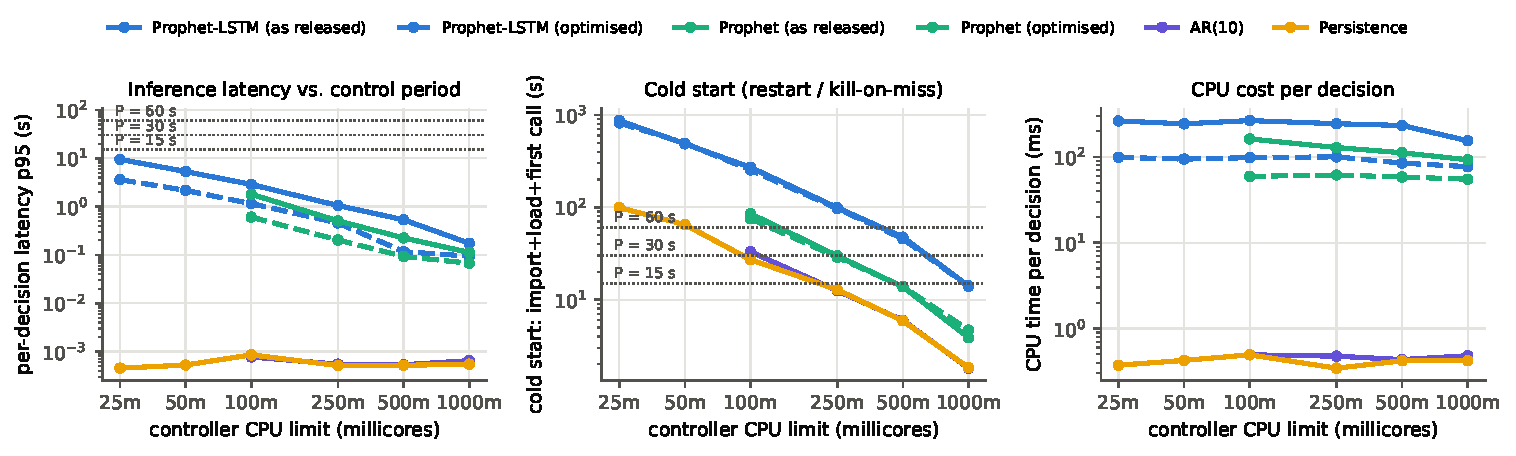
\includegraphics[width=\textwidth]{fig_e2_overhead.pdf}
\caption{E2: p95 per-decision latency, cold start and CPU per decision as a function of the scaler's CPU limit
(FIFA models, log scales). Dotted lines: control periods 15/30/60\,s.}\label{fig:e2}
\end{figure}
\begin{table}[H]\centering\scriptsize
\resizebox{\textwidth}{!}{\begin{tabular}{llrrrrrrr}
\toprule
Forecaster & Limit & CPU/dec. (ms) & p50 (ms) & p95 (ms) & Cold start (s) & RSS (MB) & Thr. (\%) & Budget@15s (\%) \\
\midrule
Prophet-LSTM (as released) & 100m & 266 & 2649 & 2858 & 270.3 & 696 & 100 & 17.72 \\
Prophet-LSTM (as released) & 250m & 244 & 950 & 1049 & 99.1 & 700 & 94 & 6.52 \\
Prophet-LSTM (as released) & 500m & 233 & 385 & 532 & 47.5 & 699 & 60 & 3.11 \\
Prophet-LSTM (as released) & 1000m & 154 & 153 & 174 & 14.1 & 694 & 3 & 1.03 \\
Prophet-LSTM (as released) & none & 157 & 156 & 167 & 13.0 & 692 & -- & -- \\
Prophet-LSTM (optimised) & 100m & 98 & 993 & 1150 & 253.7 & 686 & 93 & 6.55 \\
Prophet-LSTM (optimised) & 250m & 100 & 314 & 458 & 96.8 & 692 & 64 & 2.68 \\
Prophet-LSTM (optimised) & 500m & 85 & 110 & 117 & 45.7 & 682 & 34 & 1.13 \\
Prophet-LSTM (optimised) & 1000m & 77 & 77 & 94 & 13.9 & 688 & 0 & 0.51 \\
Prophet-LSTM (optimised) & none & 78 & 81 & 86 & 13.1 & 690 & -- & -- \\
Prophet (as released) & 100m & 162 & 1607 & 1799 & 85.2 & 169 & 100 & 10.82 \\
Prophet (as released) & 250m & 129 & 493 & 505 & 29.8 & 169 & 70 & 3.44 \\
Prophet (as released) & 500m & 112 & 200 & 224 & 13.8 & 170 & 46 & 1.49 \\
Prophet (as released) & 1000m & 93 & 95 & 112 & 3.9 & 169 & 0 & 0.62 \\
Prophet (as released) & none & 88 & 93 & 105 & 3.8 & 170 & -- & -- \\
Prophet (optimised) & 100m & 59 & 506 & 606 & 75.1 & 171 & 73 & 3.96 \\
Prophet (optimised) & 250m & 62 & 193 & 203 & 28.8 & 170 & 49 & 1.64 \\
Prophet (optimised) & 500m & 58 & 87 & 93 & 13.8 & 170 & 29 & 0.78 \\
Prophet (optimised) & 1000m & 55 & 57 & 67 & 4.7 & 170 & 0 & 0.37 \\
Prophet (optimised) & none & 59 & 62 & 70 & 3.9 & 168 & -- & -- \\
AR(10) & 100m & 0.5 & 0.5 & 0.8 & 33.0 & 88 & 4 & 0.03 \\
AR(10) & 250m & 0.5 & 0.5 & 0.5 & 12.5 & 89 & 0 & 0.01 \\
AR(10) & 500m & 0.4 & 0.5 & 0.5 & 6.0 & 89 & 0 & 0.01 \\
AR(10) & 1000m & 0.5 & 0.5 & 0.7 & 1.8 & 89 & 0 & 0.00 \\
AR(10) & none & 0.5 & 0.5 & 0.6 & 1.8 & 89 & -- & -- \\
Persistence & 100m & 0.5 & 0.5 & 0.9 & 27.1 & 89 & 0 & 0.03 \\
Persistence & 250m & 0.3 & 0.4 & 0.5 & 12.8 & 89 & 0 & 0.01 \\
Persistence & 500m & 0.4 & 0.5 & 0.5 & 5.9 & 90 & 0 & 0.01 \\
Persistence & 1000m & 0.4 & 0.4 & 0.5 & 1.8 & 89 & 0 & 0.00 \\
Persistence & none & 0.4 & 0.4 & 0.6 & 2.1 & 90 & -- & -- \\
\bottomrule
\end{tabular}
}
\caption{E2: overhead per configuration (30 decisions each). Budget@15s is the share of the period's CPU budget
($\text{limit}\times15$\,s) used by one forecast. Thr.: share of CFS periods that were throttled.}\label{tab:e2}
\end{table}

\paragraph{Per-decision inference fits every budget.} Even at 100m, the as-released hybrid needs
266\,ms of CPU and 2.65\,s of wall time per decision (p95 2.86\,s). That is less than 20\,\% of a 15\,s period.
The late-forecast fraction is \textbf{0} for every forecaster, budget and $P\in\{15,30,60\}$\,s. The deadline
mechanism was exercised in the smoke test (\texttt{tests/smoke\_budget.py}), but it never triggered under these
conditions.

\paragraph{Throttling inflates CPU cost.} Under tight quotas the same forecast costs more CPU: for the hybrid,
157\,ms unlimited vs.\ 266\,ms at 100m. 100\,\% of CFS periods are throttled at 100m. TensorFlow and Stan spawn
threads per host core, and those threads contend inside a 10\,\% quota.

\paragraph{The binding costs are start-up, memory and re-fitting, not inference.}
\begin{itemize}
\item \textbf{Cold start.} Import, model load and first call of the hybrid take 270\,s at 100m (18 control
      periods of 15\,s), 99\,s at 250m and 48\,s at 500m. Persistence and AR(10) take 27--33\,s at 100m, almost
      all of it pandas import and data loading.
\item \textbf{Consequence for kill-on-miss.} The kill-and-restart policy is therefore dangerous below 500m. A
      single miss would leave the controller on the fallback for minutes.
\item \textbf{Memory.} The hybrid's resident set is $\approx$\,700\,MB, against 170\,MB for Prophet and
      90\,MB for the light models, independent of the CPU limit.
\item \textbf{Re-fitting} (Table~\ref{tab:refit}). Re-fitting Prophet on 7 days of data takes 64\,s at 100m,
      and \emph{one} LSTM epoch takes 136\,s. A full re-training (6--16 epochs in E1) would take 14--36\,min of
      controller time. Periodic re-training cannot share the controller's budget.
\end{itemize}

\paragraph{Implementation dominates model cost.} Disabling Prophet's uncertainty sampling, which the point
forecast does not use, and calling the LSTM directly instead of \texttt{Model.predict} reduces CPU per decision
by 50--64\,\% for the hybrid (from 266 to 98\,ms at 100m) and by 41--64\,\% for Prophet. The forecasts themselves are identical.

\begin{table}[H]\centering\small
\begin{tabular}{lrrrrr}
\toprule
Limit & Rows (7 d) & Prophet fit wall (s) & CPU (s) & LSTM 1 epoch wall (s) & CPU (s) \\
\midrule
100m & 10,080 & 64 & 5.3 & 136 & 13.4 \\
500m & 10,080 & 11 & 4.5 & 24 & 12.0 \\
1000m & 10,080 & 3 & 2.4 & 9 & 8.7 \\
\bottomrule
\end{tabular}

\caption{E2: cost of re-fitting the hybrid inside the controller budget (7-day window, FIFA).}\label{tab:refit}
\end{table}

\subsection{E3: Trace-driven scaling comparison}
\begin{figure}[H]\centering
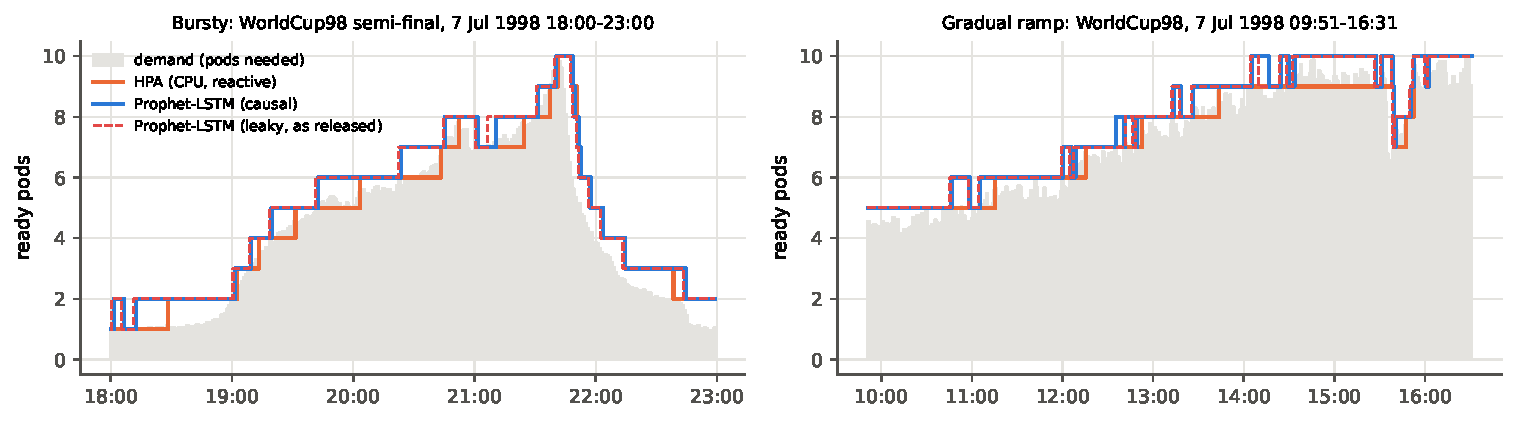
\includegraphics[width=\textwidth]{fig_e3_sim_timeseries.pdf}
\caption{E3: ready pods under the shared replica policy for HPA, the causal hybrid and the leaky hybrid
(bursty and ramp scenarios). Grey: pods needed by the demand at the 70\,\% target.}\label{fig:e3ts}
\end{figure}
\begin{figure}[H]\centering
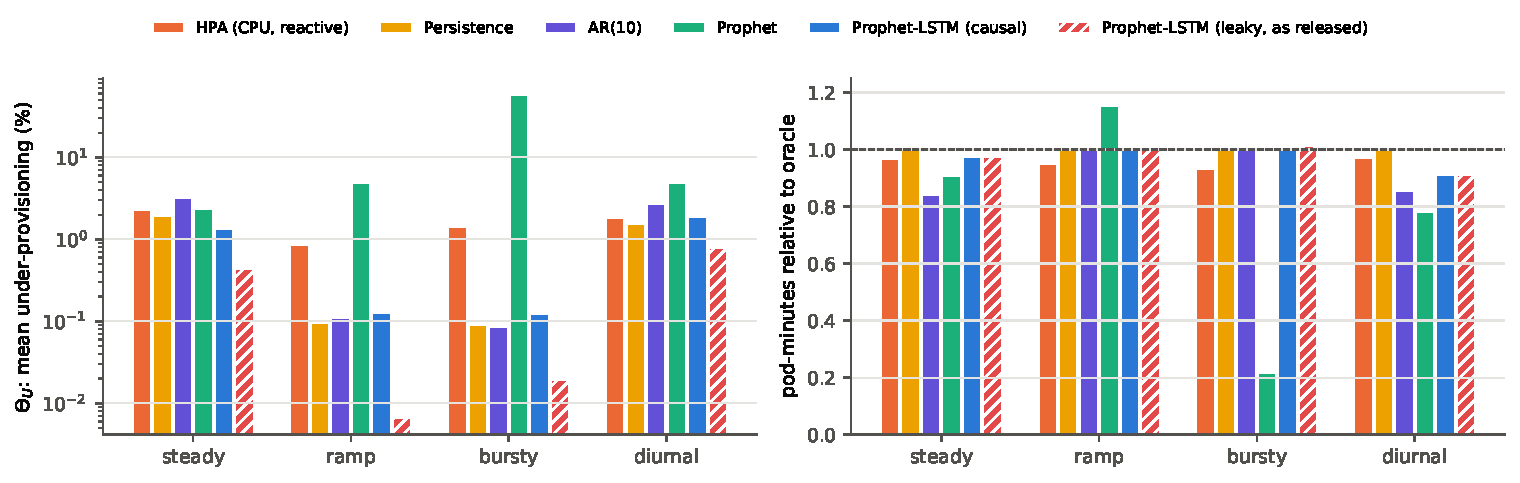
\includegraphics[width=\textwidth]{fig_e3_sim_bars.pdf}
\caption{E3: under-provisioning $\Theta_U$ (log scale) and pod-minutes relative to the oracle scaler.}\label{fig:e3bars}
\end{figure}
\begin{table}[H]\centering\scriptsize
\begin{tabular}{llrrrrrr}
\toprule
Scenario & Signal & $\Theta_U$ (\%) & $\Theta_O$ (\%) & $T_U$ (\%) & $T_O$ (\%) & mean pods & sat. (\%) \\
\midrule
steady & HPA (CPU, reactive) & 2.31 & 157.4 & 12.6 & 87.4 & 4.14 & 2.4 \\
 & Persistence & 1.92 & 164.5 & 10.7 & 89.3 & 4.29 & 1.8 \\
 & AR(10) & 3.23 & 129.8 & 17.6 & 82.4 & 3.61 & 3.6 \\
 & Prophet & 2.37 & 150.1 & 13.8 & 86.2 & 3.89 & 1.7 \\
 & Prophet-LSTM (causal) & 1.35 & 167.9 & 9.2 & 90.8 & 4.18 & 0.6 \\
 & Prophet-LSTM (leaky, as released) & 0.44 & 161.9 & 5.7 & 94.3 & 4.18 & 0.1 \\
 & Oracle & 0.00 & 153.7 & 0.0 & 99.9 & 4.29 & 0.0 \\
ramp & HPA (CPU, reactive) & 0.84 & 6.9 & 22.7 & 77.1 & 7.44 & 0.0 \\
 & Persistence & 0.10 & 11.2 & 3.7 & 96.0 & 7.81 & 0.0 \\
 & AR(10) & 0.11 & 11.1 & 4.2 & 95.5 & 7.81 & 0.0 \\
 & Prophet & 4.84 & 25.6 & 44.1 & 55.9 & 9.02 & 0.0 \\
 & Prophet-LSTM (causal) & 0.13 & 11.4 & 4.5 & 95.3 & 7.82 & 0.0 \\
 & Prophet-LSTM (leaky, as released) & 0.01 & 11.1 & 1.2 & 98.5 & 7.80 & 0.0 \\
 & Oracle & 0.00 & 11.3 & 0.0 & 99.8 & 7.83 & 0.0 \\
bursty & HPA (CPU, reactive) & 1.43 & 21.0 & 30.3 & 69.7 & 4.53 & 0.0 \\
 & Persistence & 0.09 & 31.1 & 3.7 & 96.0 & 4.85 & 0.0 \\
 & AR(10) & 0.09 & 31.3 & 3.3 & 96.3 & 4.87 & 0.0 \\
 & Prophet & 58.45 & 0.3 & 92.3 & 7.7 & 1.06 & 77.0 \\
 & Prophet-LSTM (causal) & 0.12 & 33.0 & 3.3 & 96.3 & 4.90 & 0.0 \\
 & Prophet-LSTM (leaky, as released) & 0.02 & 33.2 & 0.7 & 99.0 & 4.92 & 0.0 \\
 & Oracle & 0.00 & 31.2 & 0.0 & 99.7 & 4.86 & 0.0 \\
diurnal & HPA (CPU, reactive) & 1.84 & 102.7 & 11.8 & 87.3 & 4.30 & 1.1 \\
 & Persistence & 1.53 & 108.7 & 10.2 & 89.1 & 4.44 & 0.9 \\
 & AR(10) & 2.74 & 81.9 & 17.9 & 80.3 & 3.79 & 1.7 \\
 & Prophet & 4.82 & 62.2 & 26.5 & 71.2 & 3.46 & 4.8 \\
 & Prophet-LSTM (causal) & 1.89 & 93.0 & 12.8 & 85.7 & 4.04 & 1.2 \\
 & Prophet-LSTM (leaky, as released) & 0.77 & 88.3 & 9.7 & 88.7 & 4.04 & 0.0 \\
 & Oracle & 0.00 & 102.1 & 0.0 & 98.8 & 4.44 & 0.0 \\
\bottomrule
\end{tabular}

\caption{E3: provisioning metrics (startup delay 0). ``sat.'': share of minutes in which demand exceeded the
pods' full capacity $N C$. The oracle scaler uses the true $y_{t+1}$.}\label{tab:e3}
\end{table}

\paragraph{Request-rate scaling beats CPU-HPA on non-stationary load, but forecasting adds little.} On the
\texttt{ramp} and \texttt{bursty} scenarios, every causal request-rate scaler reduces under-provisioning
compared with the HPA:
\begin{itemize}
\item persistence, AR(10) and the causal hybrid all reach $\Theta_U\approx0.1$\,\%, against 0.84--1.43\,\% for
      the HPA;
\item time under-provisioned falls from 23--30\,\% to 3--4.5\,\%;
\item the price is 5--8\,\% more pod-minutes.
\end{itemize}
The \emph{persistence} scaler, which simply uses the last observed request rate, already captures this gain.
The improvement thus comes from the \emph{signal}: a request rate with no metric saturation and no 10\,\% CPU
tolerance band. It does not come from forecasting. On the NASA scenarios, where load is low and noisy, all
causal scalers except Prophet and AR(10) are within about 1 percentage point. The hybrid has the lowest causal
$\Theta_U$ on \texttt{steady} (1.35\,\% vs.\ 1.92\,\% persistence and 2.31\,\% HPA), but not on
\texttt{diurnal} (1.89\,\% vs.\ 1.53\,\% persistence and 1.84\,\% HPA).

\paragraph{Prophet alone is unsafe on bursty load.} Prophet's seasonal forecast misses the semi-final flash
crowd entirely. Demand exceeds full capacity in 77\,\% of minutes and $\Theta_U=58$\,\%. This is the B2 baseline
failure mode that the residual LSTM corrects.

\paragraph{Leakage also inflates scaling quality.} Driven by the leaky series, the hybrid looks 3--13$\times$
better than its causal version ($\Theta_U$ 0.02 vs.\ 0.12 on bursty; 0.44 vs.\ 1.35 on steady). An offline
evaluation of autoscaling built on the leaky forecasts would therefore overstate the benefit too. With a
one-step pod startup delay, all scalers degrade slightly and the ranking is unchanged (\texttt{results/e3\_scaling.json}).

\paragraph{Budget-induced late forecasts.} Because E2 measured no late forecasts, the budget-enforced variants
of E3 coincide with the unconstrained ones. The budget therefore affects decision quality only through cold
starts (restarts, scale-out of the controller) and the impossibility of in-budget re-training.

\subsection{E4: Live Kubernetes comparison (one repetition)}
\begin{figure}[H]\centering
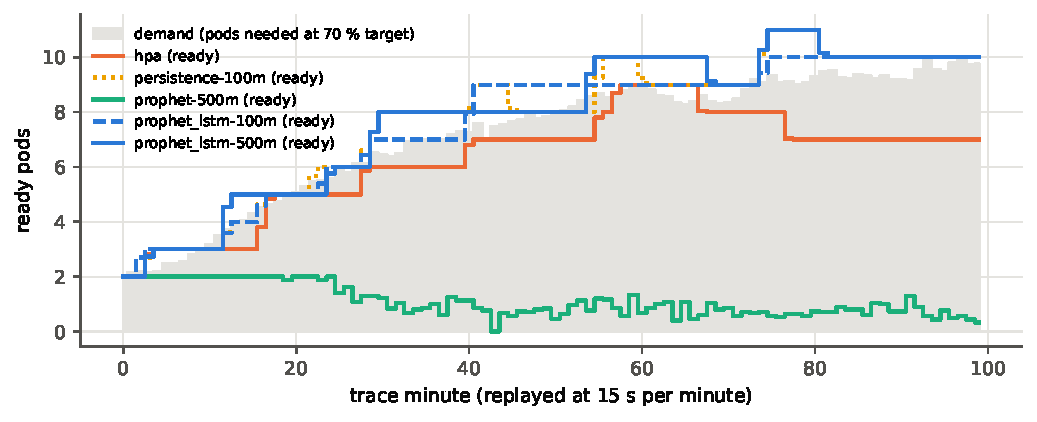
\includegraphics[width=\textwidth]{fig_e4_live.pdf}
\caption{E4: ready \texttt{work} pods during the live replay of the \texttt{bursty} slice on kind. Grey: pods
needed by the offered load at the 70\,\% target.}\label{fig:e4}
\end{figure}
\begin{table}[H]\centering\scriptsize
\resizebox{\textwidth}{!}{\begin{tabular}{lrrrrrrrrrr}
\toprule
Autoscaler & $\Theta_U$ & $\Theta_O$ & $T_U$ & $T_O$ & pod-min & SLO viol. (\%) & RMSE (rps) & CPU/dec. (ms) & p95 lat. (ms) & late (\%) \\
\midrule
hpa & 12.12 & 1.9 & 79.0 & 21.0 & 627 & 1.11 & -- & -- & -- & -- \\
persistence-100m & 0.78 & 7.1 & 19.0 & 80.0 & 763 & 0.01 & 1.63 & 1 & 2 & 0.0 \\
prophet-500m & 77.13 & 0.0 & 99.0 & 1.0 & 111 & 89.97 & 17.15 & 78 & 166 & 0.0 \\
prophet\_lstm-100m & 0.66 & 7.1 & 16.0 & 83.0 & 761 & 0.54 & 1.48 & 230 & 2587 & 0.0 \\
prophet\_lstm-500m & 0.75 & 9.9 & 14.0 & 85.0 & 781 & 0.06 & 1.42 & 158 & 333 & 0.0 \\
\bottomrule
\end{tabular}
}
\caption{E4: live results (100 trace minutes, 29{,}961 requests per run). The provisioning metrics use ready pods
$\times\,0.7C$ against the offered load. SLO viol.: share of requests that failed, timed out or took more than
500\,ms. RMSE: the scaler's live $t{+}1$ forecast against the offered load, in req/s. CPU/dec.\ and p95 lat.:
per-decision forecast cost inside the CPU-limited scaler Pod.}\label{tab:e4}
\end{table}

\paragraph{The budgeted hybrid works inside a live controller, even at 100m.} Both hybrid runs made all 100
decisions on time:
\begin{itemize}
\item \textbf{0 late forecasts and 0 fallbacks.} The p95 decision latency was 2.59\,s at 100m and 0.33\,s at
      500m, against a 15\,s deadline.
\item \textbf{CPU cost is consistent with E2.} The hybrid used 230\,ms of CPU per decision at 100m and 158\,ms
      at 500m, against 266\,ms and 233\,ms measured offline (E2 used one decision per second, so it was
      throttled more). At 100m the whole scaler container used 534\,ms of
      CPU per 15\,s period, which is 36\,\% of its quota. It was throttled for 2.8\,s per period.
\item \textbf{Cold start is the real cost.} The scaler became ready after 328\,s at 100m (22 control periods)
      and after 48\,s at 500m. Prophet alone needed 20\,s at 500m. The orchestrator waits for readiness, so
      cold start does not affect the replay itself. In production it would be a window without forecasts.
\item \textbf{Memory.} Peak container memory (cgroup, including page cache) was 0.54\,GB at 100m and 1.3\,GB
      at 500m, against 0.26\,GB for Prophet.
\end{itemize}

\paragraph{Request-rate scaling beats the CPU HPA on the flash crowd.} Against the HPA, both hybrid runs:
\begin{itemize}
\item cut $\Theta_U$ from 12.1\,\% to 0.7\,\%, and $T_U$ from 79\,\% to 14--16\,\% of minutes;
\item cut SLO violations from 1.11\,\% to 0.54\,\% (100m) and 0.06\,\% (500m);
\item cost 21--25\,\% more pod-minutes (761--781 vs.\ 627).
\end{itemize}
The HPA lagged the ramp by several minutes and scaled \emph{down} at minutes 66 and 76 while demand stayed
high (Fig.~\ref{fig:e4}). Its CPU signal saturates at the pod limit and moves inside the 10\,\% tolerance band.

\paragraph{The gain does not come from forecasting.} Measured on the observed request rate, the hybrid's live
$t{+}1$ forecast is no more accurate than persistence:
\begin{itemize}
\item at 100m: RMSE 2.23 vs.\ 2.23\,req/s;
\item at 500m: RMSE 2.00 vs.\ 2.00\,req/s.
\end{itemize}
The LSTM residual correction makes the hybrid behave like a last-value predictor. This agrees with E1 and E3:
the improvement over the HPA comes from scaling on the request rate, not from the model.

\paragraph{Prophet alone fails, as in E3.} Prophet's forecast stayed at 1.3--1.6 pods for the whole run, so the
Deployment never left its initial 2 replicas while demand rose to 10 pods' worth:
\begin{itemize}
\item the overloaded pods failed their readiness probes, and ready pods dropped below 1 (Fig.~\ref{fig:e4});
\item 54\,\% of requests failed or timed out, and 90\,\% violated the SLO.
\end{itemize}
This is the B2 failure mode predicted by the simulator. Its live forecast RMSE (5.26\,req/s on the observed
rate) is worse than persistence (4.39).

\paragraph{Caveats.} There is one run per autoscaler, on one scenario, on a single-node cluster that shares the
host with the load generator. The difference between 100m and 500m (0.54\,\% vs.\ 0.06\,\% SLO violations)
is within what run-to-run noise could produce, and it is not attributed to the budget. The deadline never
triggered, so the kill-and-fallback path was not exercised live.


%=====================================================================
\section{Troubleshooting and Corrective Actions}
\begin{itemize}
\item \textbf{KEDA HPA without the external metric.} In the first live attempt, the \texttt{ScaledObject} was
      applied together with the scaler Deployment. KEDA called \texttt{GetMetricSpec} before the gRPC server
      was listening (\texttt{connection refused}) and generated an HPA containing only a default 80\,\% CPU
      metric. It did not retry. As a result, the ``predictive'' run was silently a CPU HPA.
      \emph{Fix:} the orchestrator now applies the \texttt{ScaledObject} only after the scaler reports ready, and
      it aborts unless the generated HPA contains the \texttt{External} metric. The invalid run was discarded.
\item \textbf{Truncated per-pod target.} KEDA 2.16 used the integer \texttt{targetSize}, so a target of
      2.8\,req/s per pod became 2. That would have given the predictive scalers 40\,\% more capacity than the
      HPA. \emph{Fix:} the metric is exported in milli-requests/s (target 2800). The value was verified on the
      generated HPA before each run.
\item \textbf{Template placeholder in a comment} broke \texttt{string.Template} substitution in the first run.
      It was fixed and the affected run repeated.
\item \textbf{Noisy capacity calibration} while model training ran in parallel (3\,req/s measured as
      95--127m). Calibration and all timing experiments were repeated on an otherwise idle host.
\item \textbf{Python 3.15 on the host.} TensorFlow has no wheels for it, so an isolated Python 3.11
      environment (uv) and container images are used.
\item \textbf{Defects found in the released KEDA scaler} (in addition to F1--F6 of Cutoff~2):
      \begin{itemize}
      \item F7: \texttt{rate()} returns req/s but the model expects req/min, and the scaler multiplies by a
            \texttt{scaleFactor} of 100 instead of 60.
      \item F8: the residual is computed against Prophet's forecast for $t{+}1$ instead of $t$.
      \item F9: the pod count is truncated with \texttt{int()}.
      \end{itemize}
      Our scaler converts units explicitly, uses $r_t=y_t-\hat y^P_t$, and lets the HPA round up.
\end{itemize}

%=====================================================================
\section{Threats to Validity and Next Steps}
\begin{itemize}
\item \textbf{Single host, single repetition.} E2 and E4 have one run per configuration, and the live cluster
      shares the host with its load generator. Before the final paper we will repeat E4 (at least 3 seeds per
      autoscaler) and E2 (3 repetitions), and report confidence intervals.
\item \textbf{Time compression.} One trace minute equals 15\,s, and the HPA and Prometheus windows are scaled
      accordingly. Pod start-up (2--3\,s) is therefore relatively slower than in real time.
\item \textbf{Capacity model.} A synthetic CPU-bound service with linear CPU per request is used. Real services
      have non-linear and memory-bound behaviour.
\item \textbf{Scope of the CPU budget.} The limit is applied to the scaler Pod only. The control plane, KEDA and
      Prometheus are not budgeted.
\item \textbf{Next steps (Day 80 draft):}
      \begin{itemize}
      \item repeated live runs on all scenarios, including the light forecasters (AR(10), persistence) in KEDA;
      \item a deadline-tightening experiment ($D<P$) to locate the budget at which late forecasts start;
      \item statistical tests (paired bootstrap) on the provisioning metrics;
      \item a discussion of when, if ever, the hybrid's extra cost pays off.
      \end{itemize}
\end{itemize}


%=====================================================================
\begin{thebibliography}{9}\small
\bibitem{guruge2025} P.\,B.\ Guruge and Y.\,H.\,P.\,P.\ Priyadarshana, ``Time series forecasting-based Kubernetes autoscaling using Facebook Prophet and Long Short-Term Memory,'' \textit{Frontiers in Computer Science}, vol.\ 7, Art.\ 1509165, 2025, doi:10.3389/fcomp.2025.1509165.
\bibitem{dangquang2021} N.-M.\ Dang-Quang and M.\ Yoo, ``Deep learning-based autoscaling using bidirectional long short-term memory for Kubernetes,'' \textit{Applied Sciences}, vol.\ 11, no.\ 9, Art.\ 3835, 2021.
\bibitem{lanciano2024} G.\ Lanciano, F.\ Galli, T.\ Cucinotta, D.\ Bacciu and A.\ Passarella, ``Extending OpenStack Monasca for predictive elasticity control,'' \textit{Big Data Mining and Analytics}, vol.\ 7, no.\ 2, pp.\ 315--339, 2024.
\bibitem{imdoukh2020} M.\ Imdoukh, I.\ Ahmad and M.\,G.\ Alfailakawi, ``Machine learning-based auto-scaling for containerized applications,'' \textit{Neural Computing and Applications}, vol.\ 32, pp.\ 9745--9760, 2020.
\bibitem{joshi2024} N.\,S.\ Joshi, R.\ Raghuwanshi, Y.\,M.\ Agarwal, B.\ Annappa and D.\,N.\ Sachin, ``ARIMA-PID: container auto scaling based on predictive analysis and control theory,'' \textit{Multimedia Tools and Applications}, vol.\ 83, pp.\ 26369--26386, 2024.
\end{thebibliography}
\end{document}
